\documentclass{beamer}

\usetheme{Antibes}
%\usetheme{split}
% this is a template for slides using beamer package
% adapted from slides written by Ramon Medrado
% first version: Ana Bazzan
\usecolortheme[RGB={120,0,0}]{structure}
\setbeamertemplate{blocks}[rounded][shadow=true]
\usepackage[utf8]{inputenc}   % pacote para acentuao
\usepackage{amsmath}

%% Listagens de código
\usepackage{listings}
\usepackage{color}

\setbeamertemplate{footline}[frame number]
\setbeamertemplate{navigation symbols}{}

\definecolor{codegreen}{rgb}{0,0.6,0}
\definecolor{codegray}{rgb}{0.5,0.5,0.5}
\definecolor{codepurple}{rgb}{0.58,0,0.82}
\definecolor{backcolour}{rgb}{0.95,0.95,0.92}
 
\lstdefinestyle{mystyle}{
    % backgroundcolor=\color{backcolour},   
    commentstyle=\color{codegreen},
    keywordstyle=\color{magenta},
    numberstyle=\tiny\color{codegray},
    stringstyle=\color{codepurple},
    basicstyle=\scriptsize,
    breakatwhitespace=false,         
    breaklines=false,                 
    captionpos=b,                    
    keepspaces=true,                 
    numbers=left,                    
    numbersep=3pt,                  
    showspaces=false,                
    showstringspaces=false,
    showtabs=false,                  
    tabsize=2
}
\lstset{style=mystyle}

\beamertemplateballitem

\begin{document}
\title
{Implementing a mobility scenario using SDN and Ryu Framework}


\author
{Iulisloi Zacarias \\ Prof. Dr. Luciano Paschoal Gaspary}

\institute
{
  Instituto de Informática\\
  Universidade Federal do Rio Grande do Sul (UFRGS)
}

\date[CMP166]
{CMP182 – Redes de Computadores I, 2016/I}

% UFRGS Logo
\logo{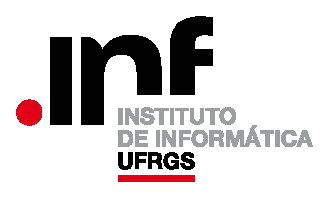
\includegraphics[scale=0.3]{images/inf}}


% If you wish to uncover everything in a step-wise fashion, uncomment
% the following command: 

%\beamerdefaultoverlayspecification{<+->}


% Slide de Título (Capa)
\frame[plain]{\titlepage}

% Slide de Resumo (Outline)
\frame{
	\frametitle{Outline}
	\tableofcontents
}

\section{Introduction}

\subsection{Scenario}

% -------------------------------- Slide 01 --------------------------------
\begin{frame}{Scenario Caracterization}
\begin{itemize}
  \item Proposed mobility scenario
  \item A stream video server
  \item Clients play the video streamed by the server
  \item Hosts can disconnect and connect from switches / access points 
\end{itemize}
\end{frame}


% \section{Celular Automaton}

% \subsection{Definition}

% -------------------------------- Slide 02 --------------------------------
\begin{frame}{Scenario Diagram}
	\begin{figure}
	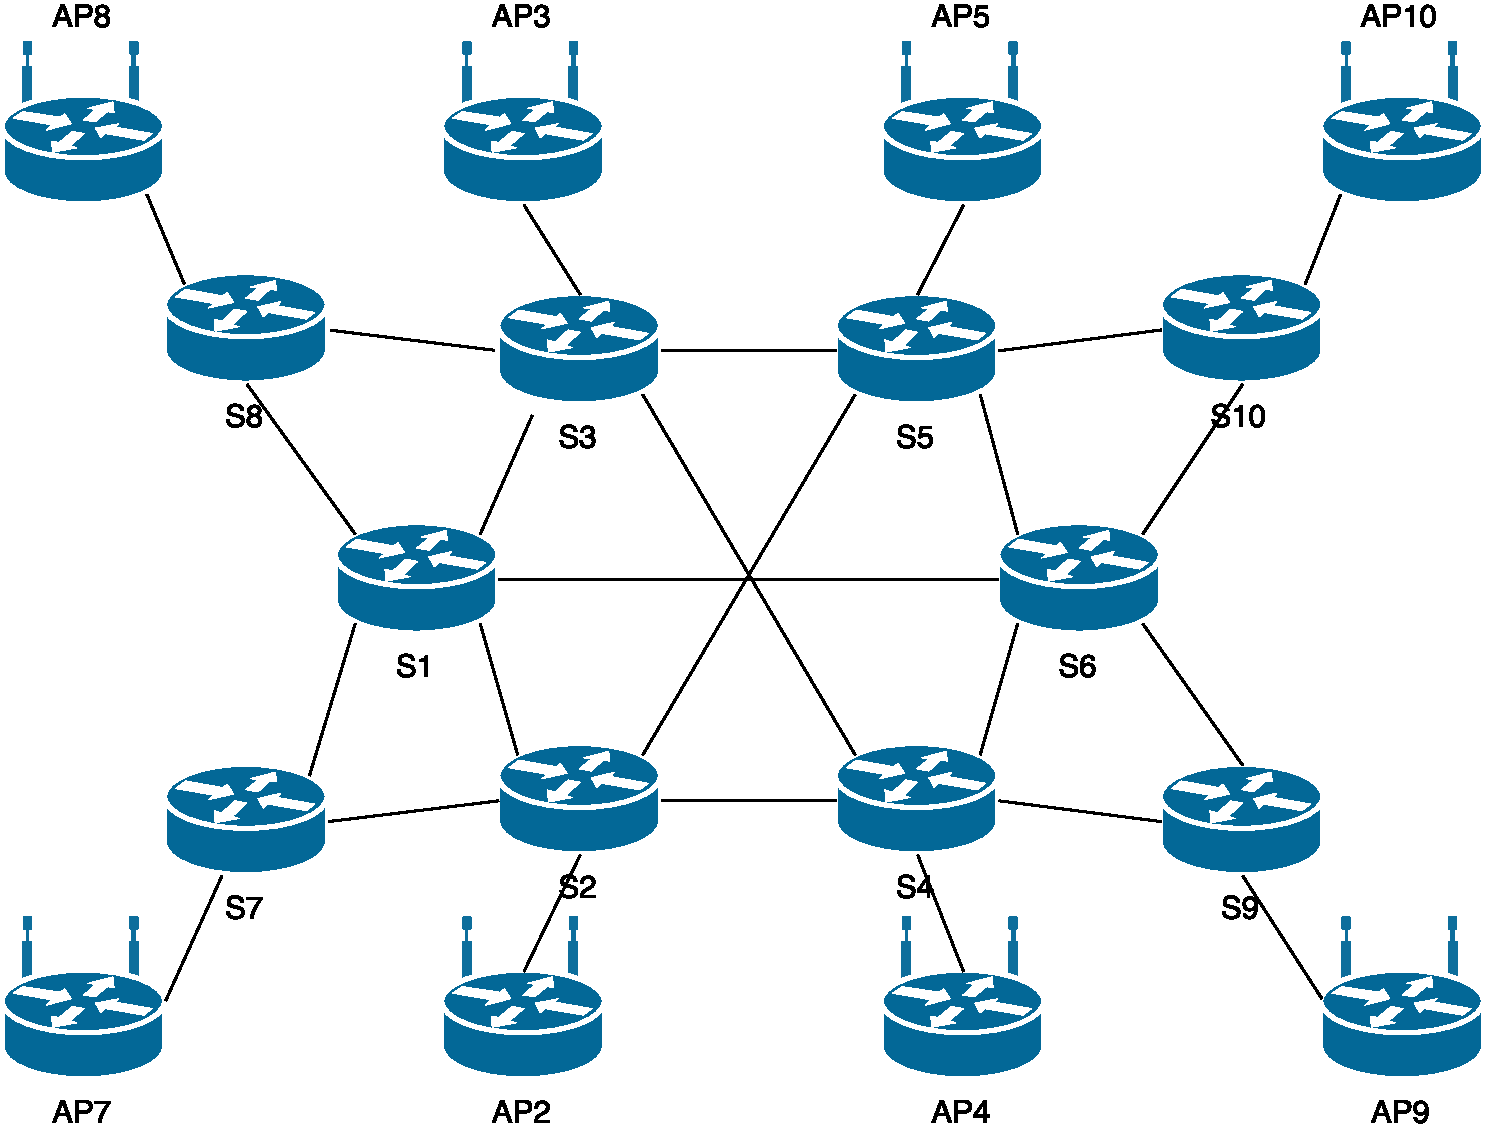
\includegraphics[scale=0.3]{images/scenario.pdf}
	\caption{\scriptsize Overview of proposed scenario}
	\end{figure}
\end{frame}


\subsection{Basic principles}
% -------------------------------- Slide 03 --------------------------------
\begin{frame}{Basic principles (1/2)}
\begin{itemize}
  \item Spatial structure is the \emph{first} most important principle (e.g.: a matrix or a vector)
  \item Each cell is a location representing an individual
  \item These set of positions is called ``world'' or ``celular world''
  \item Can represent, for example, a model of how people live in the city
\end{itemize}
\end{frame}

% -------------------------------- Slide 04 --------------------------------
\begin{frame}{Basic principles (2/2)}
\begin{itemize}
  \item Each automaton has neighbors on sides
  \item The social self-organization concept arises from local interactions among individuals (neighborhood)
  \item In cellular automaton models, we can give precise meaning to what we mean of local interaction
  \item Local interaction is the \emph{second} important principle of a cellular automaton
  \item An individual can only interact with others in specified distance around
\end{itemize}
\end{frame}

% -------------------------------- Slide 05 --------------------------------
\begin{frame}{Types of neighborhoods}
\begin{itemize}
  \item There are many different types of neighborhoods
  \item The most common are:
  \begin{itemize}
    \item Von Neumann Neighborhood (a)
    \item Moore Neighborhood (b)
  \end{itemize}
  \item Moore neighborhood can be customized, for example, a 5x5 Moore neighborhood (c)
\end{itemize}
\begin{center}
  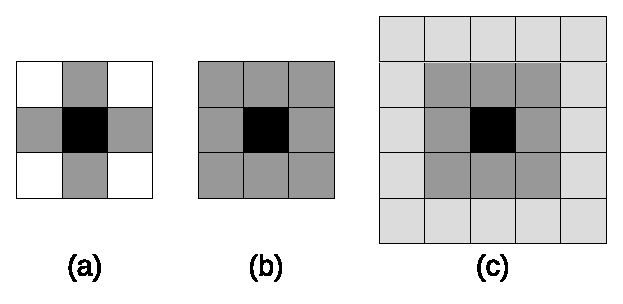
\includegraphics[scale=0.50]{images/neighbourhood}
\end{center}
\end{frame}

% -------------------------------- Slide 06 --------------------------------
\begin{frame}{Neighborhood and interaction}
\begin{itemize}
  \item Different kind of neighborhood models distinct individuals interactions
  \item Taking the example of spread a rumor, in the Moore neighborhood the rumor will spread faster than in Von Neumann neighborhood
  \item The way you model the neighborhood express how local or global the interaction is
\end{itemize}
\end{frame}

% -------------------------------- Slide 07 --------------------------------
\begin{frame}{Modeling the interaction}
  \begin{beamerboxesrounded}[shadow=true]{How can we model the interaction?}
    R: Once more, two basic principles
  \end{beamerboxesrounded}
\end{frame}

% -------------------------------- Slide 08 --------------------------------
\begin{frame}{First Principle: The cell state}
\begin{itemize}
  \item The agents in the cells have a state
  \item The states can represent the opinion, ethnicity
  \item Typically, the states are modeled as a number (e.g. 1, 2, 3) or a binary value (e.g. ``On'' of ``Off'')
\end{itemize}
\end{frame}

% -------------------------------- Slide 09 --------------------------------
\begin{frame}{Second Principle: The rules}
\begin{itemize}
  \item Agents can change their states
  \item How they update their ``states'' depends on both, the own state and the states of their neighbors
\end{itemize}
\end{frame}

\subsection{Interaction}
% -------------------------------- Slide 10 --------------------------------
\begin{frame}{How state changes are modeled?}
\begin{itemize}
  \item Time is discrete in cellular automaton models
  \item All agents can change their states every step (tick) at the same time
  \begin{itemize}
    \item They take their own state and the state of neighbors in previous time, and they all change to a new state
  \end{itemize}
  \item One agent at the time can change its state (e.g.: a randomly selected agent will change its state)
\end{itemize}
\end{frame}

% -------------------------------- Slide 11 --------------------------------
\begin{frame}{State change dynamics}
\begin{itemize}
  \item Influence dynamics
  \begin{itemize}
    \item Agents do not change their location but change their state
  \end{itemize}
  \item Migration dynamics
  \begin{itemize}
  \item Agent may move to another place in the world, depending on the current state of the neighborhood
  \end{itemize}
\end{itemize}
\end{frame}


\section{Why study cellular automaton}
% -------------------------------- Slide 12 --------------------------------
\begin{frame}{How many automaton rules are there?}
\begin{itemize}
  \item There are many rules (really?!)
  \begin{itemize}
    \item How many rules we can create with a one-dimension world, two states, and a neighborhood or three cells
    \item Number of Rules = ${S}^{N} = {2}^{3} = 8$
    \item There are two possible ending for each rule ($S = 2$), thus:
      \begin{equation*}
       {S^S}^{N} = {2^2}^{3} = 256 ~rules
      \end{equation*}
    \item If you spent 1 minute examining each rule, you will work for 4:15h
    % \item Considering a neighborhood of five cells: Rules = 2^2^5 = 4,294,967,296
  \end{itemize}
\end{itemize}
\end{frame}

\section{Cellular automaton and Chaos}
\subsection{Cellular automaton behavior}
% -------------------------------- Slide 13 --------------------------------
\begin{frame}{From chaos emerge organization}
\begin{itemize}
  \item Random start states can produce similar patterns
\end{itemize}

  \begin{figure}[ht]
	  \begin{minipage}[b]{0.45\linewidth}
	    \centering
	    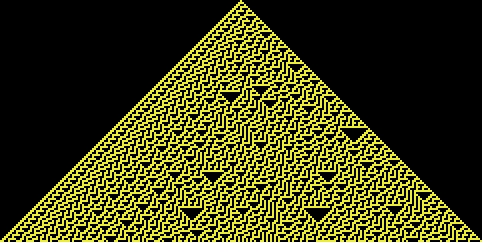
\includegraphics[width=\textwidth]{images/single_start.png}
		  \caption{\scriptsize Single point start state}
    \end{minipage}
    \hspace{0.5cm}
    \begin{minipage}[b]{0.45\linewidth}
	    \centering
	    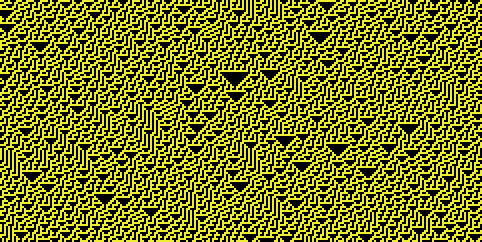
\includegraphics[width=\textwidth]{images/rand_start.png}
	    \caption{\scriptsize Random start state}
    \end{minipage}
  \end{figure}
\end{frame}


\section{Examples and application}
% -------------------------------- Slide 14 --------------------------------
\begin{frame}{The Game of Life}
\begin{itemize}
  \item Undoubtedly, the best-known cellular automata model is ``Game of Life''
  \item It was proposed by John Conway
  \item Game of life can form different, interesting, patterns
\end{itemize}
\end{frame}



% -------------------------------- Slide 15 --------------------------------
\begin{frame}{Interesting, but where we can use that?}
\begin{itemize}
  \item Computer processors
  \item Cryptography (Rule 30)
  \item Random number generation
  \item Error correction coding (hardware based)
  \item Fluid dynamics
  \item Social interaction
  \item Eletric power systems
\end{itemize}
\end{frame}

\section{References}
\begin{frame}{References}
\begin{thebibliography}{Schroeder, 1991}
\bibitem[M. R. Schroeder, 1991]{Schroeder1991}
  M.~R.~Schroeder.
  \newblock Cellular Automata.
  \newblock {\em Fractals, Chaos, Power Laws: Minutes from an Infinite Paradise}, p. 371--390
  \newblock Dover Publications, 1991.  
    
\bibitem[Peak, 1994]{Peak1994}
  D.~Peak,~M.~Frame.
  \newblock Some Call It Life
  \newblock {\em Chaos Under Control: The Art and Science of Complexity}, p. 301--337, 1994.
  
\bibitem[Peak, 1994]{Peak1994}
  D.~Barone~\textit{et al.}
  \newblock Autômatos Celulares
  \newblock {\em Sociedades artificiais: a nova fronteira da inteligência nas máquinas}, p. 41--60.
  \newblock Bookman, 1991.  
\end{thebibliography}
\end{frame}

\end{document}




